\documentclass{article}\usepackage[]{graphicx}\usepackage[]{color}
% maxwidth is the original width if it is less than linewidth
% otherwise use linewidth (to make sure the graphics do not exceed the margin)
\makeatletter
\def\maxwidth{ %
  \ifdim\Gin@nat@width>\linewidth
    \linewidth
  \else
    \Gin@nat@width
  \fi
}
\makeatother

\definecolor{fgcolor}{rgb}{0.345, 0.345, 0.345}
\newcommand{\hlnum}[1]{\textcolor[rgb]{0.686,0.059,0.569}{#1}}%
\newcommand{\hlstr}[1]{\textcolor[rgb]{0.192,0.494,0.8}{#1}}%
\newcommand{\hlcom}[1]{\textcolor[rgb]{0.678,0.584,0.686}{\textit{#1}}}%
\newcommand{\hlopt}[1]{\textcolor[rgb]{0,0,0}{#1}}%
\newcommand{\hlstd}[1]{\textcolor[rgb]{0.345,0.345,0.345}{#1}}%
\newcommand{\hlkwa}[1]{\textcolor[rgb]{0.161,0.373,0.58}{\textbf{#1}}}%
\newcommand{\hlkwb}[1]{\textcolor[rgb]{0.69,0.353,0.396}{#1}}%
\newcommand{\hlkwc}[1]{\textcolor[rgb]{0.333,0.667,0.333}{#1}}%
\newcommand{\hlkwd}[1]{\textcolor[rgb]{0.737,0.353,0.396}{\textbf{#1}}}%
\let\hlipl\hlkwb

\usepackage{framed}
\makeatletter
\newenvironment{kframe}{%
 \def\at@end@of@kframe{}%
 \ifinner\ifhmode%
  \def\at@end@of@kframe{\end{minipage}}%
  \begin{minipage}{\columnwidth}%
 \fi\fi%
 \def\FrameCommand##1{\hskip\@totalleftmargin \hskip-\fboxsep
 \colorbox{shadecolor}{##1}\hskip-\fboxsep
     % There is no \\@totalrightmargin, so:
     \hskip-\linewidth \hskip-\@totalleftmargin \hskip\columnwidth}%
 \MakeFramed {\advance\hsize-\width
   \@totalleftmargin\z@ \linewidth\hsize
   \@setminipage}}%
 {\par\unskip\endMakeFramed%
 \at@end@of@kframe}
\makeatother

\definecolor{shadecolor}{rgb}{.97, .97, .97}
\definecolor{messagecolor}{rgb}{0, 0, 0}
\definecolor{warningcolor}{rgb}{1, 0, 1}
\definecolor{errorcolor}{rgb}{1, 0, 0}
\newenvironment{knitrout}{}{} % an empty environment to be redefined in TeX

\usepackage{alltt}

\usepackage{float}

% Set the margins on the page to not be so large
\addtolength{\oddsidemargin}{-.875in}
\addtolength{\evensidemargin}{-.875in}
\addtolength{\textwidth}{1.75in}
\addtolength{\topmargin}{-.875in}
\addtolength{\textheight}{1.75in}

% Take off page numbering
\pagenumbering{gobble}
\IfFileExists{upquote.sty}{\usepackage{upquote}}{}
\begin{document}

\title{%
  2.5.1: R - Multiple Predictors \\
  \smallskip
  \large Stat 5100: Dr. Bean
}
\date{}

\maketitle

\textbf{Example: } (Exercises 6.15-6.17) A hospital administrator is studying the relation between patient satisfaction ($Y$, an index) and a patient's age ($X_1$, in years), severity of illness ($X_2$, an index), and anxiety level ($X_3$, an index). Data are reported for 46 randomly selected patients. For all index variables, higher values indicate more (satisfaction, severity, anxiety).

\begin{knitrout}
\definecolor{shadecolor}{rgb}{0.969, 0.969, 0.969}\color{fgcolor}\begin{kframe}
\begin{alltt}
\hlcom{# Input the data and take a look at the first few observations}
\hlkwd{library}\hlstd{(stat5100)}
\hlkwd{data}\hlstd{(patient)}
\hlkwd{head}\hlstd{(patient)}
\end{alltt}
\begin{verbatim}
##   satisfaction age severity anxiety
## 1           48  50       51     2.3
## 2           57  36       46     2.3
## 3           66  40       48     2.2
## 4           70  41       44     1.8
## 5           89  28       43     1.8
## 6           36  49       54     2.9
\end{verbatim}
\begin{alltt}
\hlcom{# Look at the scatterplot matrix}
\hlkwd{pairs}\hlstd{(} \hlopt{~} \hlstd{satisfaction} \hlopt{+} \hlstd{age} \hlopt{+} \hlstd{severity} \hlopt{+} \hlstd{anxiety,} \hlkwc{data} \hlstd{= patient,}
       \hlkwc{main} \hlstd{=} \hlstr{"Patient satisfaction data"}\hlstd{)}
\end{alltt}
\end{kframe}

{\centering 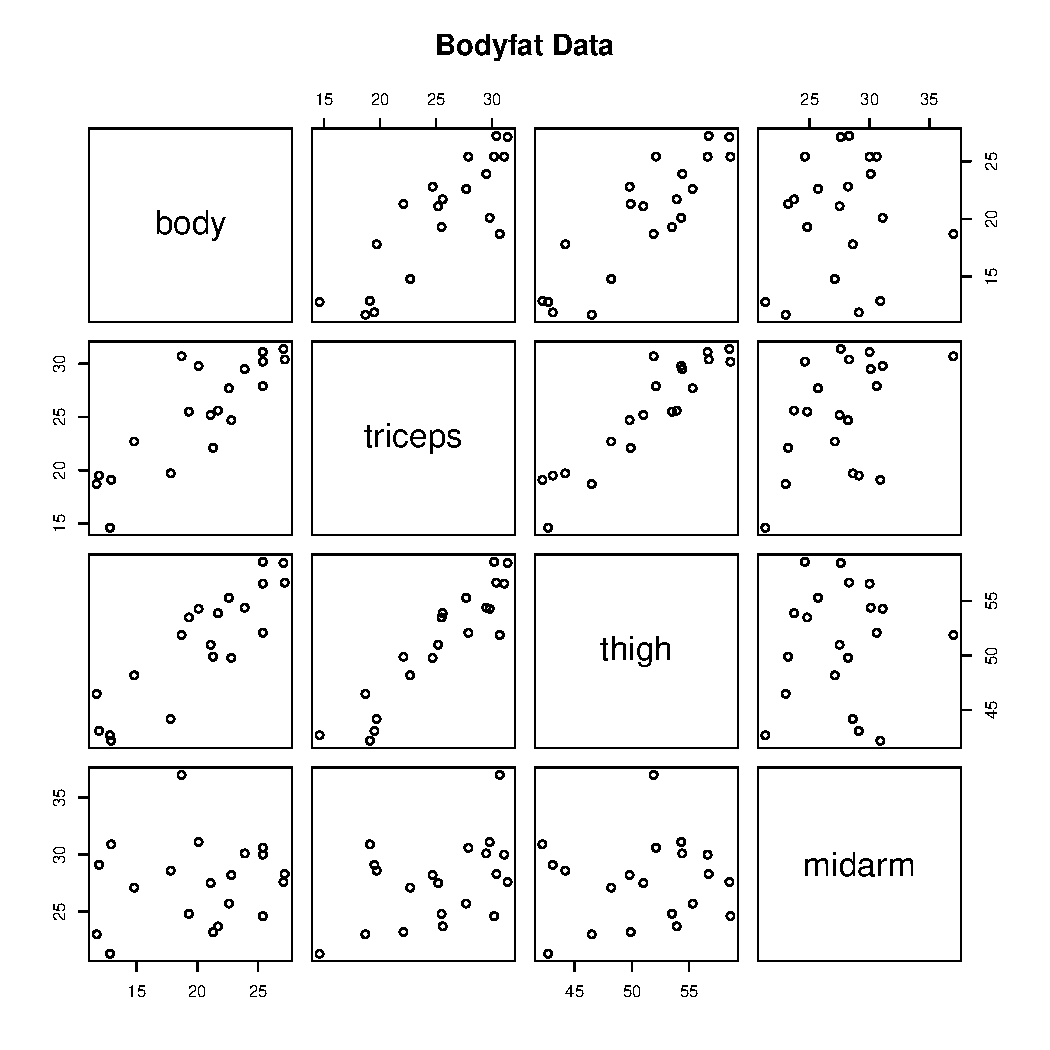
\includegraphics[width=0.6\textwidth]{figure/unnamed-chunk-1-1} 

}



\end{knitrout}

\begin{knitrout}
\definecolor{shadecolor}{rgb}{0.969, 0.969, 0.969}\color{fgcolor}\begin{kframe}
\begin{alltt}
\hlcom{# Fit a regression model}
\hlstd{patient_lm} \hlkwb{<-} \hlkwd{lm}\hlstd{(satisfaction} \hlopt{~} \hlstd{age} \hlopt{+} \hlstd{severity} \hlopt{+} \hlstd{anxiety,} \hlkwc{data} \hlstd{= patient)}
\hlkwd{summary}\hlstd{(patient_lm)}
\end{alltt}
\begin{verbatim}
## 
## Call:
## lm(formula = satisfaction ~ age + severity + anxiety, data = patient)
## 
## Residuals:
##      Min       1Q   Median       3Q      Max 
## -18.3524  -6.4230   0.5196   8.3715  17.1601 
## 
## Coefficients:
##             Estimate Std. Error t value Pr(>|t|)    
## (Intercept) 158.4913    18.1259   8.744 5.26e-11 ***
## age          -1.1416     0.2148  -5.315 3.81e-06 ***
## severity     -0.4420     0.4920  -0.898   0.3741    
## anxiety     -13.4702     7.0997  -1.897   0.0647 .  
## ---
## Signif. codes:  0 '***' 0.001 '**' 0.01 '*' 0.05 '.' 0.1 ' ' 1
## 
## Residual standard error: 10.06 on 42 degrees of freedom
## Multiple R-squared:  0.6822,	Adjusted R-squared:  0.6595 
## F-statistic: 30.05 on 3 and 42 DF,  p-value: 1.542e-10
\end{verbatim}
\begin{alltt}
\hlcom{# Check model assumptions}
\hlstd{stat5100}\hlopt{::}\hlkwd{visual_assumptions}\hlstd{(patient_lm)}
\end{alltt}
\end{kframe}

{\centering 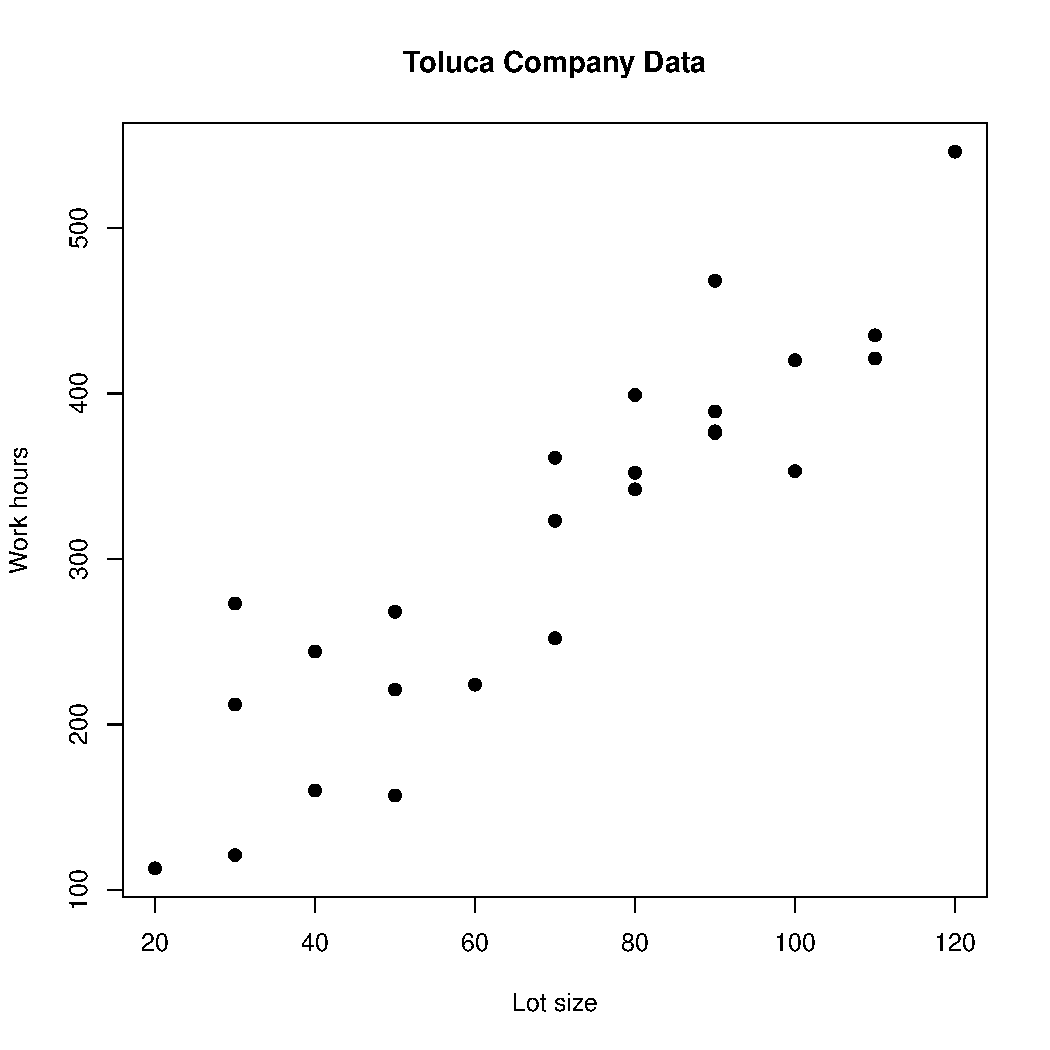
\includegraphics[width=0.6\textwidth]{figure/unnamed-chunk-2-1} 

}



\end{knitrout}

\begin{knitrout}
\definecolor{shadecolor}{rgb}{0.969, 0.969, 0.969}\color{fgcolor}\begin{kframe}
\begin{alltt}
\hlcom{# Numerical assumptions}
\hlstd{stat5100}\hlopt{::}\hlkwd{brown_forsythe_lm}\hlstd{(patient_lm)}
\end{alltt}
\begin{verbatim}
## [1] "Brown-forsythe test for constant variance in the residuals:"
## [1] "T-statistic: -0.1236, p-value: 0.9022"
\end{verbatim}
\begin{alltt}
\hlstd{stat5100}\hlopt{::}\hlkwd{cor_normality_lm}\hlstd{(patient_lm)}
\end{alltt}
\begin{verbatim}
## Correlation test of normality:
##                   resid expected_norm
## resid         1.0000000     0.9885077
## expected_norm 0.9885077     1.0000000
## 
## Total observations: 46
## Make sure to consult with table B.6 for your final result.
\end{verbatim}
\begin{alltt}
\hlcom{# Joint 90% intervals for beta1, beta2, and beta3}
\hlcom{# Because we don't care about the intercept term, we will set our confidence}
\hlcom{# level to 0.86668 which corresponds to a 90% confidence interval for just the}
\hlcom{# non-interept betas.}
\hlstd{stat5100}\hlopt{::}\hlkwd{coefficient_confidence_lm}\hlstd{(patient_lm,} \hlkwc{confidence} \hlstd{=} \hlnum{0.86668}\hlstd{,} \hlkwc{simul} \hlstd{=} \hlnum{TRUE}\hlstd{)}
\end{alltt}
\begin{verbatim}
## lower.est and upper.est are the 96.667% confidence limits.
## The Bonferroni adjustment for simultaneous confidence levels was made.
##                Estimate Std. Error    t value     Pr(>|t|)  lower.est
## (Intercept) 158.4912517 18.1258887  8.7439162 5.260955e-11 118.606836
## age          -1.1416118  0.2147988 -5.3147960 3.810252e-06  -1.614258
## severity     -0.4420043  0.4919657 -0.8984452 3.740702e-01  -1.524531
## anxiety     -13.4701632  7.0996608 -1.8972967 6.467813e-02 -29.092339
##               upper.est
## (Intercept) 198.3756674
## age          -0.6689661
## severity      0.6405229
## anxiety       2.1520128
\end{verbatim}
\begin{alltt}
\hlcom{# Simultaneous 90% prediction limits on two new patients (with Scheffe and Bonferroni)}
\hlcom{# with profiles:}
\hlcom{#       1. age = 35, severity = 45, anxiety = 2.2}
\hlcom{#       2. age = 42, severity = 61, anxiety = 1.8}
\hlstd{two_new_patients} \hlkwb{<-} \hlkwd{data.frame}\hlstd{(}\hlkwc{age} \hlstd{=} \hlkwd{c}\hlstd{(}\hlnum{35}\hlstd{,} \hlnum{42}\hlstd{),}
                               \hlkwc{severity} \hlstd{=} \hlkwd{c}\hlstd{(}\hlnum{45}\hlstd{,} \hlnum{61}\hlstd{),}
                               \hlkwc{anxiety} \hlstd{=} \hlkwd{c}\hlstd{(}\hlnum{2.2}\hlstd{,} \hlnum{1.8}\hlstd{))}
\hlstd{stat5100}\hlopt{::}\hlkwd{simul_prediction_limits}\hlstd{(patient_lm, two_new_patients,} \hlkwc{confidence} \hlstd{=} \hlnum{0.90}\hlstd{)}
\end{alltt}
\begin{verbatim}
##   age severity anxiety     yhat se_yhat_pred  S_lower  S_upper  B_lower
## 1  35       45     2.2 69.01029     10.40495 46.05533 91.96524 48.01224
## 2  42       61     1.8 59.33500     12.67149 31.37972 87.29028 33.76291
##    B_upper
## 1 90.00833
## 2 84.90709
\end{verbatim}
\begin{alltt}
\hlcom{# Would we need a transformation?}
\hlstd{MASS}\hlopt{::}\hlkwd{boxcox}\hlstd{(patient_lm)}
\end{alltt}
\end{kframe}

{\centering 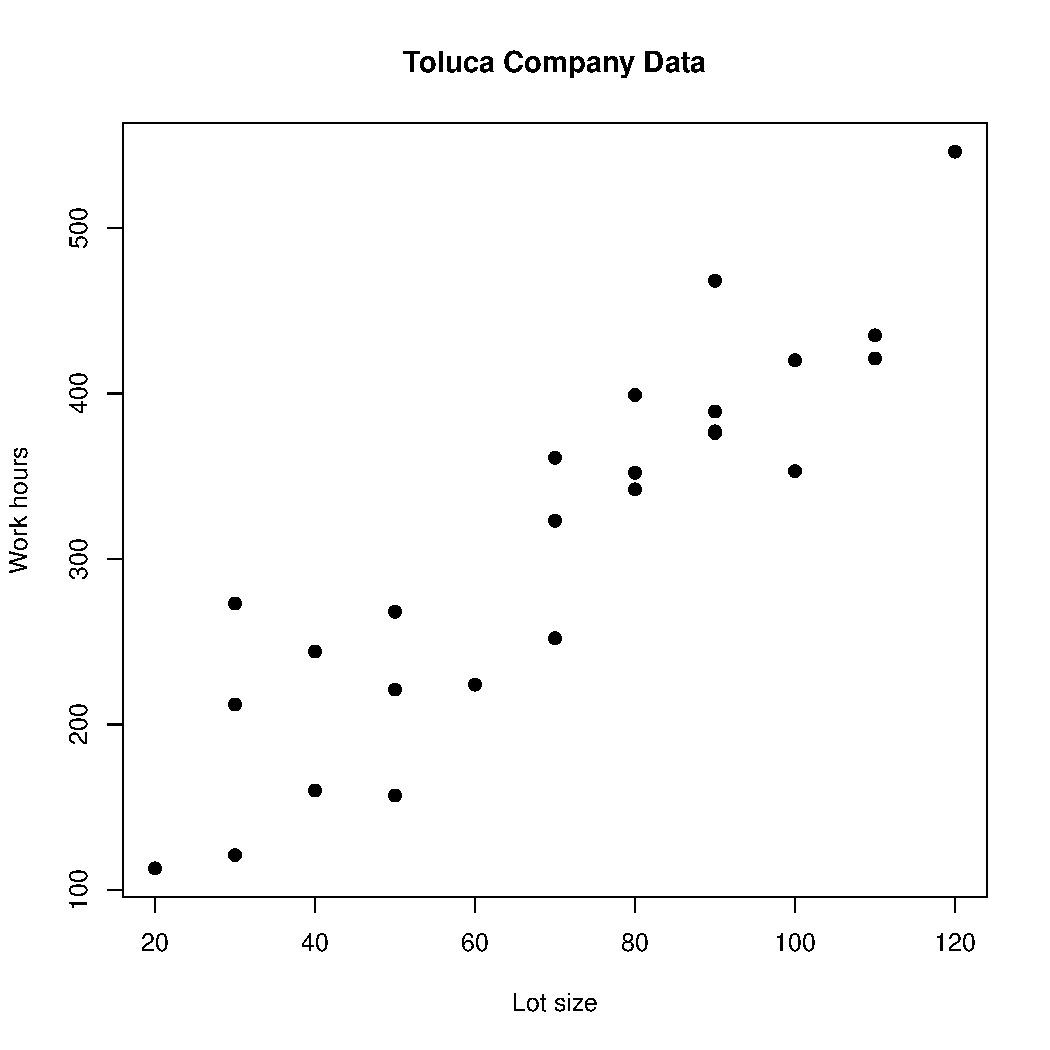
\includegraphics[width=0.6\textwidth]{figure/unnamed-chunk-3-1} 

}



\end{knitrout}

This plot above tells us that if we wanted to, we could try a square root transform on the response variable.

\end{document}
